% !TeX encoding = UTF-8
% !TeX spellcheck = en_US
% !TeX root = report1.tex

\section{Results}
%Now we focus on using the integration to solve the problem established in the introduction.
Now we will present the results obtained of using the Monte Carlo integration and the variational
method to find the ground state energy on each of the problems already established. In every case
we will compare
our results with the reference values found in \cite{JosBook}.

\subsection{Harmonic Oscillator}
Two simulations were performed with 50 iterations, a damping factor of $\gamma = 10^{-5}$,
an initial value of $\alpha_i = 3$  and 1,000 test points over a domain with length 4,
subdivided into 20 sub-domains for the adaptive grid. In the final iteration we obtained an
error in the energy of $err(E)=E_{MC}-E_{REF}\simeq 1.63\cdot 10^{-9}$,
and a error in the parameter of $err(\alpha)=\alpha - \alpha_{REF} \simeq 7.6455\cdot 10^{-6}$. In figure \ref{fig:Ho_it}
we show the values obtained for the energy and for $\alpha$ as a function of every iteration performed,
om which the parameter $\alpha$ is changing according to \ref{eq:minimizer},
for two different values of $\alpha_i$. We can see how  convergence values in both energy and $\alpha$ are
reached with a small number of iterations, which shows that the methods used are efficient. In figure
 \ref{fig:Ho_rel} we can see how the energy behaves as a function on $\alpha$ where there is a clear
minimum value at $0.5$ where each of the executions of our program meet each other.
\begin{figure}
	\begin{center}
		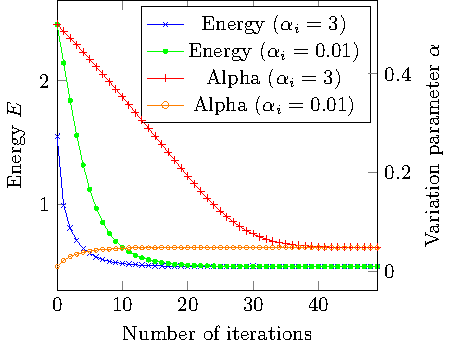
\includegraphics[scale=0.9]{graphs/ho-e-alpha-iterations.pdf}
		\caption{
			Energy and $\alpha$ obtained during every iteration for two different values $\alpha_i$.
			%Calculated $E$ as a function of $\alpha$ using two different starting values for$\alpha_0$. Notice that $\alpha$ converges monotonically (increasing or decreasing) while this is not necessarily true for the energy due to the integration not being exact. Nonetheless, a very accurate result can be found: $E_{\alpha_0 = 0.5} =  $ and $E_{\alpha_0 = 0.5} =  $.
			}
		\label{fig:Ho_it}
	\end{center}
\end{figure}
\begin{figure}
	\begin{center}
		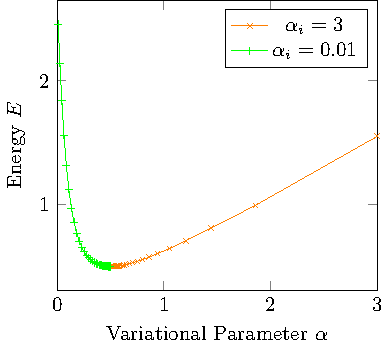
\includegraphics[scale=0.9]{graphs/ho-e-alpha.pdf}
		\caption{
			Energy as a function of $\alpha$ for two initial values of $\alpha_i$.
			%Calculated $E$ as a function of $\alpha$ using two different starting values for$\alpha_0$. Notice that $\alpha$ converges monotonically (increasing or decreasing) while this is not necessarily true for the energy due to the integration not being exact. Nonetheless, a very accurate result can be found: $E_{\alpha_0 = 0.5} =  $ and $E_{\alpha_0 = 0.5} =  $.
		}
		\label{fig:Ho_rel}
	\end{center}
\end{figure}


\subsection{Hydrogen Atom}
Using the parameters
$\gamma = 5\cdot 10^{-4}$, $\alpha_i = 3 \text{~/~}0.01$ with 5,000
test points over $7$ boxes, about 160 iterations were needed to reach convergence
values of $\alpha \approx 1$ and $E_{MC} \approx - 1/2$, where the error obtained is
$err(\alpha) = \alpha-\alpha_{REF} \simeq 5 \cdot 10^{-10}$. That is, within 160
iterations we can estimate the value $\alpha=1$ up to ten digits and find the appropriate energy for it.


\subsection{Helium Atom}

Similarly to the previous case we calculated $E$ as a function of $\alpha$
using two different starting values for $\alpha_i$, see figure~\ref{fig:He_it}.
The values found for the energy after just 50 iterations are
$E_{\alpha_i = 0.01} =  $ and $E_{\alpha_i = 0.5} =  $, which
compare well with the optimum value achieved by this method
of $-2.8781 \pm 0.0005$, the Hartree-Fock value of $-2.8617$,
the DFT value of $-2.83$ and the exact value of $-2.9307$ (see \cite{JosBook}). %TODO

\begin{figure}
  \begin{center}
  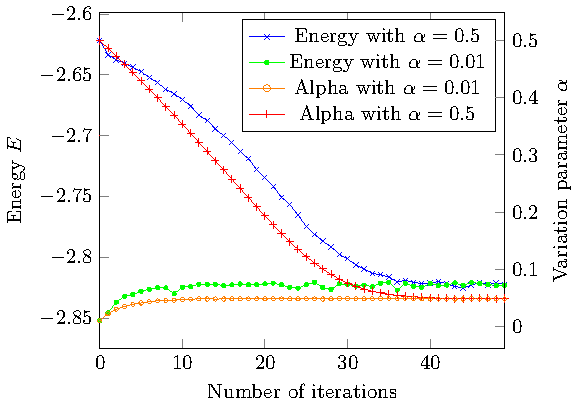
\includegraphics[scale=1 ]{graphs/he-e-alpha-iterations.pdf}
  \caption{
	Value of energy and $\alpha$ for two different $\alpha_i$
  	% Calculated $E$ as a function of $\alpha$ using two different starting values for$\alpha_0$.
		%  Notice that $\alpha$ converges monotonically (increasing or decreasing) while this is not necessarily
		%   true for the energy due to the integration not being exact. Nonetheless, a very accurate result
		% 	 can be found: $E_{\alpha_0 = 0.5} =  $ and $E_{\alpha_0 = 0.5} =  $
  	%TODO: This was already mentioned in the text. I should only be in one place!
  	}
  \label{fig:He_it}
  \end{center}
\end{figure}
